\documentclass[10pt,onecolumn,twoside,letterpaper]{article}
\usepackage[text={7in,9.5in},centering]{geometry}
\usepackage[spanish,es-nodecimaldot]{babel}

\usepackage{hyperref}

\usepackage{multicol}

\usepackage{harvard}% bibliographystyle: apsr, agsm, dcu, kluwer, nederlands

\usepackage{graphicx}
\usepackage{amssymb}
\usepackage{fancyhdr}
\usepackage{color}
\usepackage{colortbl}
\definecolor{gray}{cmyk}{0.0,0.0,0.0,0.60}

%\usepackage{auto-pst-pdf}
%\usepackage{pst-all}

%\usepackage[numbered]{mcode}
%\usepackage{lipsum}

\pagestyle{fancy}
\fancyhf{}
\fancyhead[RO]{\small{\textcolor{gray}{\textsc{Hacia un framework de locomoci\'on b\'ipeda evolutiva y flexible}}}}
\fancyhead[LO]{
\includegraphics[scale=0.05]{../../images/unlogo.png}}
\fancyhead[LE]{
\includegraphics[scale=0.05]{../../images/unlogo.png}\quad\small{\textcolor{gray}{\textsc{Linea de investigaci\'on: Robotica Evolutiva en Caminadores}}}}
\fancyfoot[CO,CE]{\thepage}
\fancyfoot[LO,RE]{\scriptsize{\textcolor{gray}{\emph{Version 0.2}}}}

\title{\vspace{-0.8cm}
\includegraphics[scale=0.12]{../../images/unescudobn.png}\\\vspace{-0.0cm}
  \LARGE \textbf{Modelos din\'amicos de locomoci\'on b\'ipeda}}
\author{J.A. Castillo-Le\'on\thanks{jacastillol@unal.edu.co} \and R.E. Ram\'irez-Heredia\thanks{reramirezh@unal.edu.co}}
\date{}

\begin{document}
\maketitle
\begin{abstract}\small
  Este trabajo esta enfocado a herramientas de simulaci\'on que soporten modelos de caminadores, donde los comportamientos emergentes de locomoci\'on de los seres humanos a lo largo de su evoluci\'on puedan ser estudiados, se requiere buena programaci\'on en MATLAB y buenos fundamentos de m\'ecanica como punto de partida.
\end{abstract}
%\begin{multicols}{2}
\section{Descripci\'on:}
Basados en el modelo general de \cite{Grizzle2014} (ver la Figura \ref{fig:grizmodelo}.), que propone un modelo general basado en la formulaci\'on de Lagrange. Este modelo sirve para explorar diferentes temas concernientes en la rob\'otica b\'ipeda.
\section{Objetivo:}
El objetivo principal de este trabajo es desarrollar una colecci\'on de ejemplos a modo de librer\'ia que permita la construicci\'on r\'apida de modelos b\'ipedos, en el cual se pueda comprobar distintas configuraciones mecanicas, leyes de control y proponer diferntes tipos de actuaci\'on. Bastaria entonces con generar ejemplos de cada una de los siguientes enfoques PWD, ZMP, FRI, CoM, HZD, SLIP, para asegurar un equilibrio din\'amico. Se necesita que sea desarrollado sobre C++ y el motor de juegos Open Dynamic Engine ODE ademas debe ser validado su resultado con MATLAB-SimMechanics.
%\end{multicols}
\begin{figure}[!ht]
  \centering
  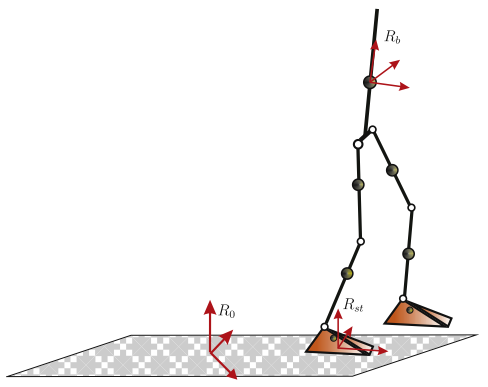
\includegraphics[scale=0.4]{../../images/GeneralBipedModel.png}
  \caption{Modelo Din\'amico General}
  \label{fig:grizmodelo}
\end{figure}
%\nocite{*}
\bibliographystyle{nederlands}% apsr, agsm, dcu, kluwer, nederlands
\bibliography{../../review/review/library}
\end{document}
